\section{Merging changes form a branch to the master\label{sec:pull_requests}}

\textbf{Before you consider this} you need to make sure the following has been checked otherwise, you will waste developers time and test patience. In brief summary you have to check that the your new code doesn't break any of the existing unit-tests or auto-differentiation code, so you need to build all of the below commands before considering merging changes.

\begin{enumerate}
\item \texttt{doBuild archive} this will build all the autodiff librarys.
\item \texttt{doBuild modelrunner}
\item Enter the directory  \texttt{BuildSystem\textbackslash Casal2\textbackslash Casal2 - -unittest} to check all the unit-tests pass.
			
\end{enumerate}


\textbf{only once the above is done, should you consider the remaining section}. This section describes how to merge changes from a branch to the master repository. This is under the assumptions that the contributor has followed the rules laid out in Section~\ref{sec:build_rules}. 

This section is the opposite to Section~\ref{sec:maintain_repo} (where we pulled changes from the master repository into a branch). Here we are merging changes from a branch into the master, which will be incorporated into the next publicly available compiled version of \CNAME. From this example we can see from Figure~\ref{fig:fork_merge1} that our branch is 109 commit ahead and 844 commits behind (underlined in blue) that we want to incorporate into the master repository.

To incorporate these changes into the master you need to click on the \enquote{pull request} button. This will prompt a comparison of the changes that you are submitting for inclusion into the master.
\clearpage
\begin{figure}[!ht]
	\centering
	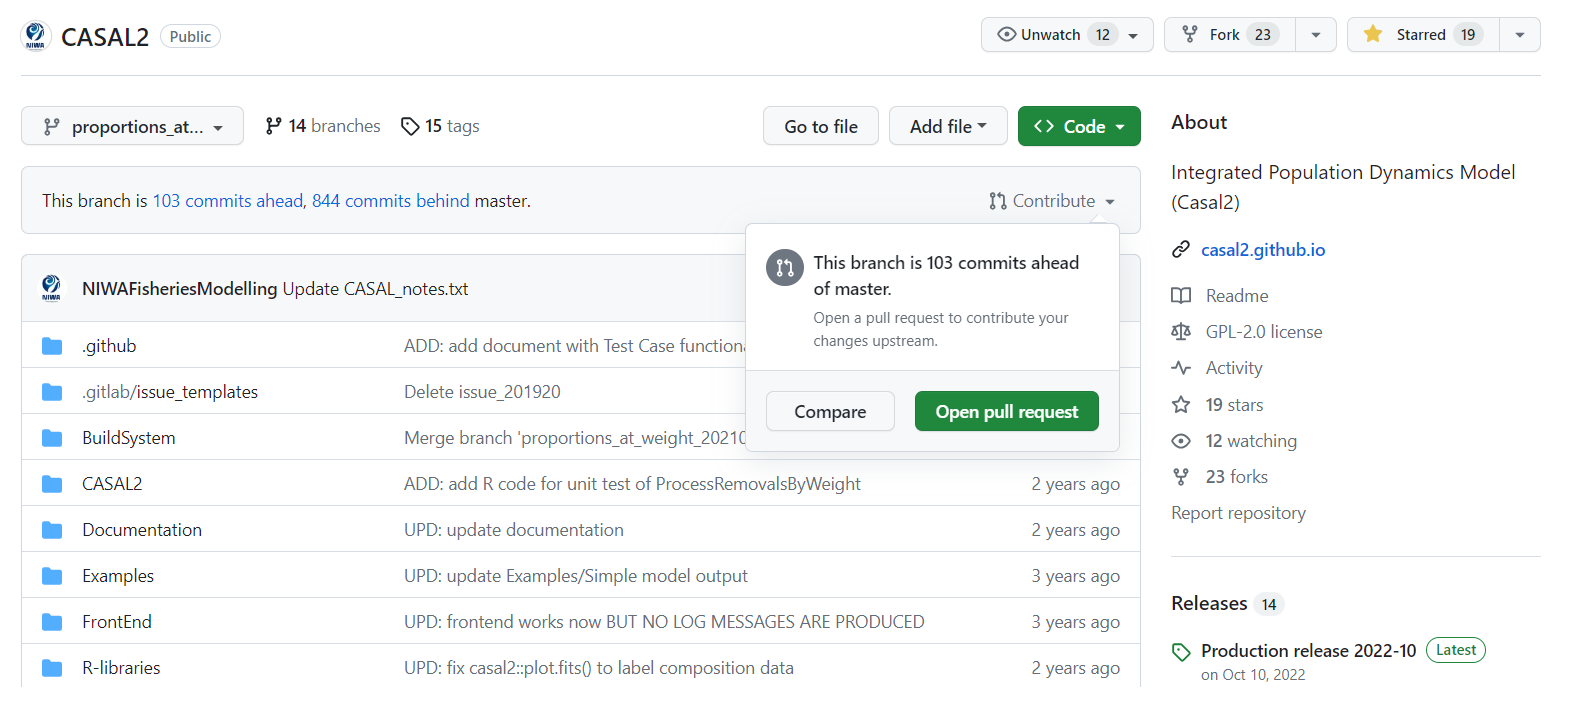
\includegraphics[scale=0.4]{Figures/create_pull_request.png}
	\caption{}\label{fig:fork_merge1}
\end{figure}

We can see that there are 10 files changed over three commits. A the top left corner there is a green button with \enquote{create pull request} click that button. This will open a pull request on the master repository as shown in Figure~\ref{fig:fork_merge2}
\begin{figure}[!ht]
	\centering
	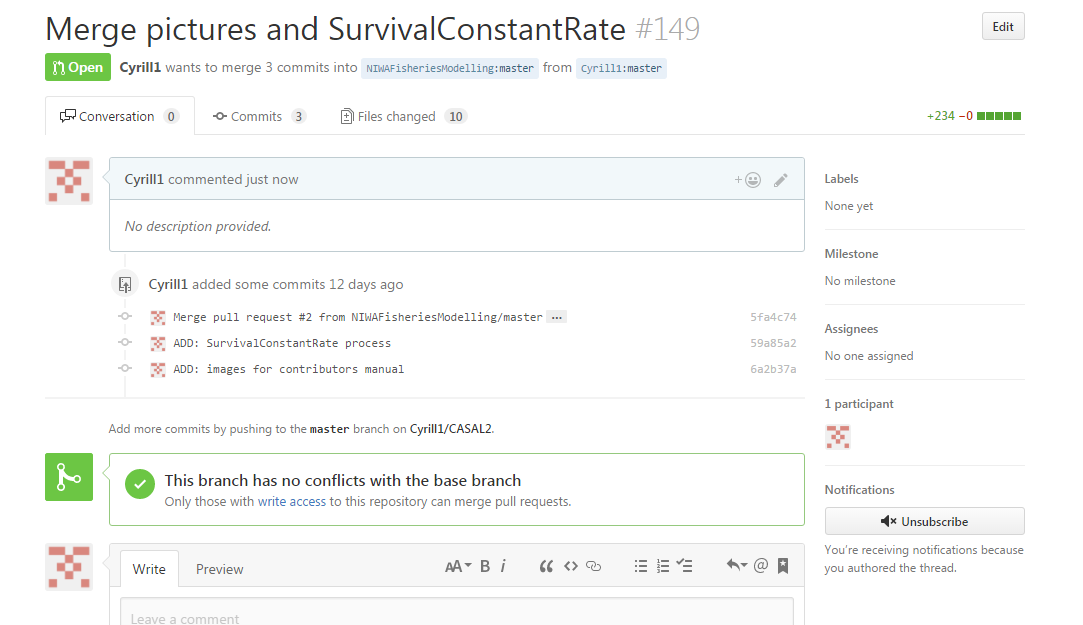
\includegraphics[scale=0.6]{Figures/Pull_request1.png}
	\caption{}\label{fig:fork_merge2}
\end{figure}

This will notify the maintainers of the master repository that a contributor is requesting a merge of the forked code into the master. Maintainers are able to look through the proposed code changed and have conversations with the contributors if they need clarification. But at this point we are just waiting for the maintainers to accept the changes which then get incorporated into \CNAME\ which then makes you a legend.

If you make it this far, we thank you for your development and contributions of this tool and we hope that you get great use out of it =)


